\subsection{Logistic Regression}

We have applied logistic regression to our data. For logistic regression, we calculate a value for each data object. This value can be used to estimate the likelihood of the object to be CHD positive.

\begin{figure}
	\begin{subfigure}
	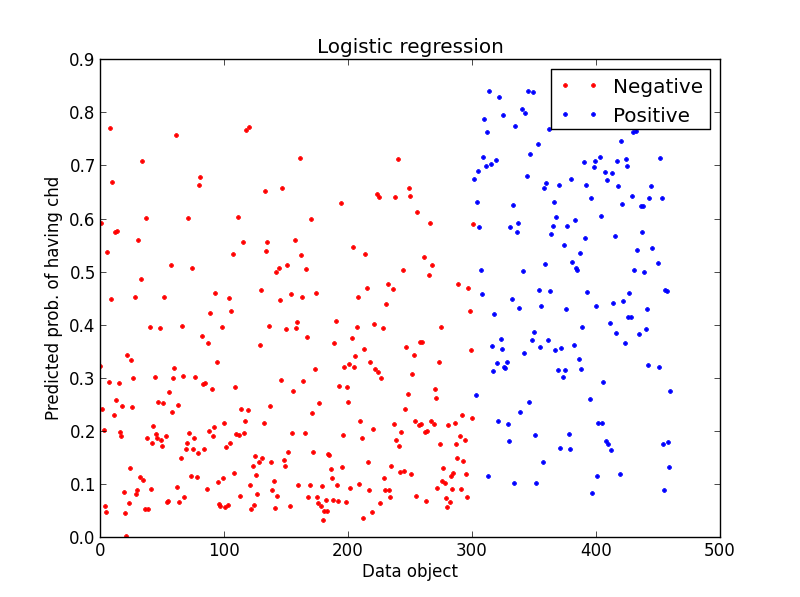
\includegraphics[scale=0.3]{logisticregressionX.png}
	\caption{Looking at all attributes.}
	\label{logicalRegressionResultX}
	\end{subfigure}

	\begin{subfigure}
	\includegraphics[scale=0.3]{logisticregressionXad.png}	
	\caption{Looking at attributes selected by forward selection.}
	\label{logicalRegressionResultXad}
	\end{subfigure}

	\begin{subfigure}
	\includegraphics[scale=0.3]{logisticregressionXPA.png}
	\caption{Looking at all principal components.}
	\label{logicalRegressionResultXPA}
	\end{subfigure}

	\begin{subfigure}
	\includegraphics[scale=0.3]{logisticregressionX2PA.png}
	\caption{Looking at two most important principal components.}
	\label{logicalRegressionResultX2PA}
	\end{subfigure}
\caption{This figure shows results of performing logical regression for different input.}
\label{logicalRegressionResults}
\end{figure}

Se Figure \ref{logicalRegressionResults} to see output for our different input